
% \section{FPGA~\cite[Section~B.6.5]{stephen2022fundamentals}}
% 
% \includegraphics[width=0.5\linewidth]{./media/FPGA.png}
% \includegraphics[width=0.5\linewidth]{./media/LUT.png}\\
% \includegraphics[width=0.5\linewidth]{./media/FF-LUT.png}
% \includegraphics[width=0.5\linewidth]{./media/programmed-FPGA.png}
% 
% 
% \begin{definition}[Random Access Memory (RAM)] Structure of a RAM is as follows:\\
%   \includegraphics[width=0.3\linewidth]{./media/memory-array.png}
%   \includegraphics[width=0.3\linewidth]{./media/memory-array-32kb.png}
%   \includegraphics[width=0.3\linewidth]{./media/SRAM-cell.png}\\
%   \includegraphics[width=0.7\linewidth]{./media/SRAM.png}
% \end{definition}
% 
% \begin{definition}[Read Only Memory (ROM)] Structure of a ROM is as follows:\\
%   \includegraphics[width=\linewidth]{./media/rom.png}
% \end{definition}


\begin{definition}[Fan-in]
  The fan-in of a logic gate is number of  inputs to a logic gate.~\cite[Section~B.8.9]{stephen2022fundamentals}
\end{definition}
\includegraphics[width=0.3\linewidth]{./media/fan-in.png}

\begin{remark}[Fan-in]
  The fan-in of a gate is limited by the propagation delay $t_p$. Higher the
  fan-in, higher the $t_p$. The output
  voltage thresholds like $V_{OL}$ and $V_{OH}$ also limit fan-in. Higher the
  fan-in, higher is $V_{OL}$ (and lower is the $V_{OH}$).
\end{remark}

\begin{example}
  Implement an OR gate with fan-in of 7 using OR gates with fan-in of 3.
\end{example}
\vspace{5em}

\begin{definition}[Fan-out]
  The fan-out of a logic gate is the maximum number of other gates that can be connected
  to output of a gate.~\cite[Section~B.8.9]{stephen2022fundamentals}
\end{definition}
\includegraphics[width=0.5\linewidth]{./media/fan-out.png}

% \begin{definition}[Programmable Logic Array (PLA) ] Structure of a PLA:\\
%   \includegraphics[width=0.7\linewidth]{./media/AND-OR-PLA.png}~\cite[Section~B.6.1]{stephen2022fundamentals}
%   %\includegraphics[width=0.7\linewidth]{./media/NOR-NOR-PLA.png}
% \end{definition}
% 
% \begin{definition}[Programmable Array Logic (PAL)] Structure of a PAL:\\
%   \includegraphics[width=0.7\linewidth]{./media/AND-OR-PAL.png}~\cite[Section~B.6.2]{stephen2022fundamentals}
% \end{definition}
% 
% \begin{example}
%   What is the difference between PLA and PAL?
% \end{example}
% \vspace{5em}

\section{Timing parameters for sequential circuit~\cite[Section~3.5]{harris2022digital}}

\includegraphics[width=0.6\linewidth]{./media/ff-timings.png}\\
\begin{definition}[Setup time $t_{su}$ of a latch/flip-flop]
  Time for which input must be stable before the clock edge.
\end{definition}

\begin{definition}[Hold time $t_h$ of a latch/flip-flop]
  Time for which input must be stable after the clock edge.
\end{definition}

\begin{definition}[Clock-to-Q contamination delay $t_{ccq}$ of a latch/flip-flop]
  Time taken to influence (contaminate) the Q output after the clock edge.
\end{definition}

\begin{definition}[Clock-to-Q propagation delay $t_{ccq}$ of a latch/flip-flop]
  Time taken for Q output to stabalize  after the clock edge.
\end{definition}
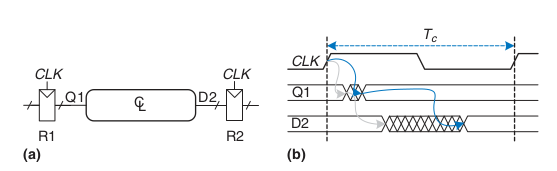
\includegraphics[width=0.8\linewidth]{./media/fig3.38.png}

\begin{definition}[Setup Time Constraint]
  $T_c > t_{pcq} + t_{pd} + t_{setup}$\\
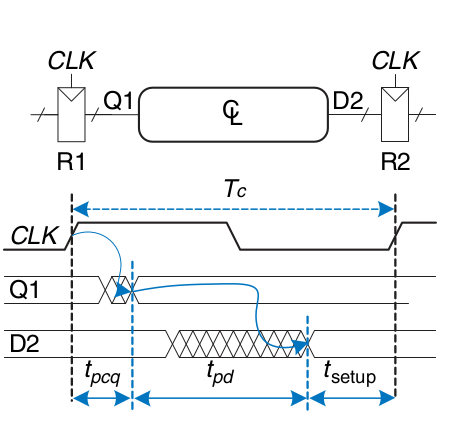
\includegraphics[width=0.8\linewidth]{./media/fig3.39.png}
\end{definition}

\begin{definition}[Hold Time Constraint]
  $t_{ccq} + t_{cd} \ge t_{hold}$\\
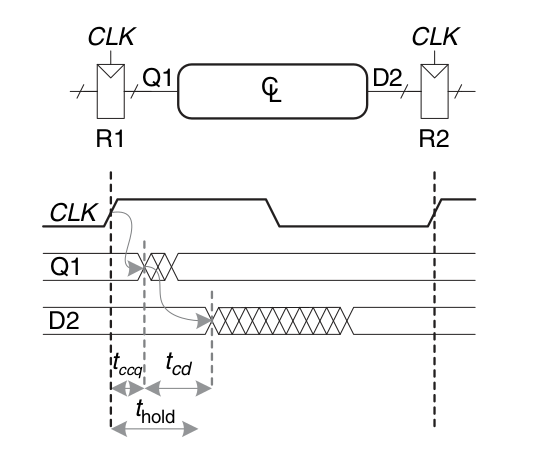
\includegraphics[width=0.8\linewidth]{./media/fig3.40.png}
\end{definition}

